\section{Introduction}
\label{paperB:sec:introduction}

%\renewcommand{\thefootnote}{\fnsymbol{footnote}}
In recent years, computer vision-based assistive technologies have been developed for supporting people with visual impairments.
Such technologies exist in the form of mobile applications, e.g., Microsoft's Seeing AI~\citeB{B:seeingAImicrosoft} and Aipoly Vision~\citeB{B:aipolyvision}, and as wearable artificial vision devices, e.g., Orcam MyEye~\citeB{B:orcam}, Transsense~\citeB{B:transsense}, and the Sound of Vision system~\citeB{B:caraiman2017soundofvision}. These products can support people with visual impairments in many different situations, such as reading text documents, describing the user's environment, and recognizing people the user may know. 
%Such technologies exist in the form of mobile applications, e.g., Microsoft's Seeing AI ({\small \url{https://www.microsoft.com/en-us/seeing-ai/}}) and Aipoly Vision ({\small \url{https://www.aipoly.com/}}), and as wearable artificial vision devices, e.g., Orcam MyEye ({\small \url{https://www.orcam.com/en/}}), Transsense ({\small \url{https://www.transsense.ai/}}), and the Sound of Vision system~\citeB{caraiman2017soundofvision}. These products can support people with visual impairments in many different situations, such as reading text documents, describing the user's environment, and recognizing people the user may know. 
In this paper, we focus on an application that is essential for assistive vision, namely visual support when shopping for grocery items considering a large range of eatable objects, including fruits, vegetables, and refrigerated products, e.g., milk and juice packages.

Grocery shopping with low vision capabilities can be difficult for various reasons. For example, in grocery store sections for raw groceries, the items are often stacked in large bins as shown in Figure \ref{fig:dataset_figures}a-f. Additionally, similar items are usually stacked next to each other, and therefore, items are can be misplaced into neighboring bins. Humans can distinguish between groceries without vision to some degree, e.g., by touch and smell, but it requires prior knowledge about texture and fragrance of food items. 
Furthermore, packaged items, e.g., milk, juice, and yoghurt cartons, can only be differentiated with the help of visual information (see Figure \ref{fig:dataset_figures}g-i). 
Such items usually have barcodes, that are readable using the existing assistive vision devices described above. 
Even if using a barcode detector is a clever solution, it can be inconvenient and exhausting always having to detect barcodes of packaged items.
Therefore, an assistive vision device that relies on natural images would be of significant value for a visually impaired person in a grocery store. 

%%% Figure 1 and 2


\begin{figure}[t] 
	\centering
	\begin{minipage}[b]{0.47\textwidth}
    	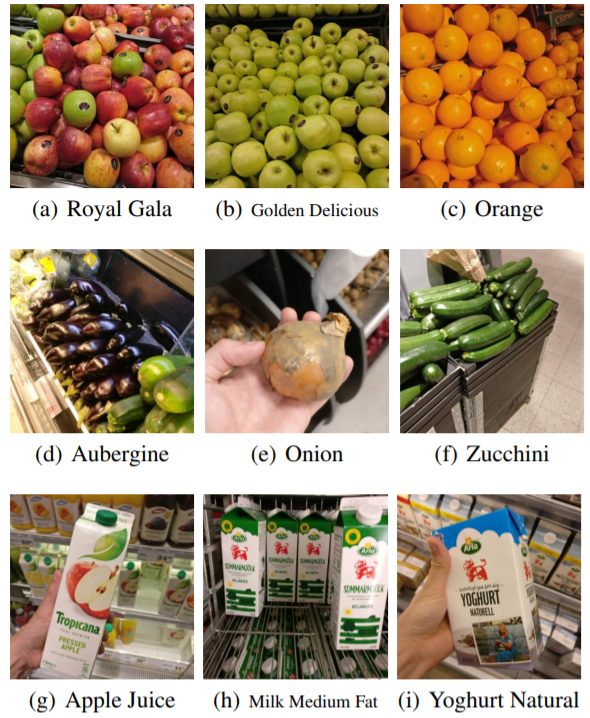
\includegraphics[scale=0.5]{PaperB/figures_and_tables/figure1.png}
		\caption{Examples of natural images in our dataset, where each image has been taken inside a grocery store. Image examples of fruits, vegetables, and refrigerated products are presented in each row respectively.}
		\label{fig:dataset_figures}
	\end{minipage}
	\hspace{10pt}
	%\vspace{-10mm}
	\begin{minipage}[b]{0.47\textwidth}
		\centering
	    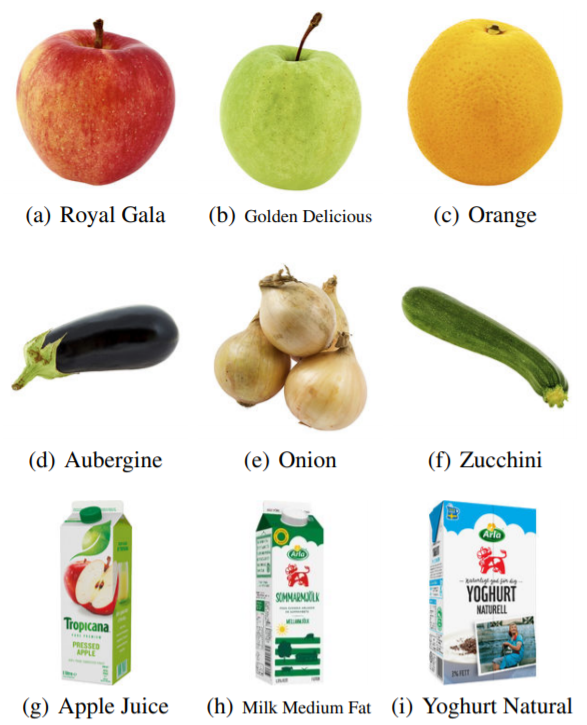
\includegraphics[scale=0.5]{PaperB/figures_and_tables/figure2.png}
		\caption{Examples of iconic images downloaded from a grocery shopping website, which corresponds to the target items in the images in Figure \ref{fig:dataset_figures}. \newline}
		\label{fig:iconic_image_figures}
	\end{minipage} 
	\vspace{-2mm}
\end{figure}



\begin{comment}

\begin{figure}
    \centering
    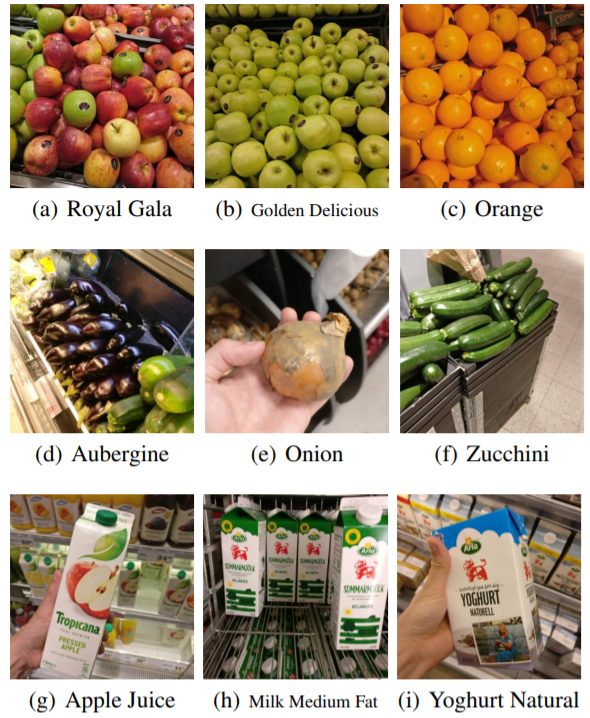
\includegraphics[scale=0.5]{PaperB/figures_and_tables/figure1.png}
    \caption{Examples of natural images in our dataset, where each image has been taken inside a grocery store. Image examples of fruits, vegetables, and refrigerated products are presented in each row respectively.}
    \label{fig:dataset_figures}
\end{figure}

\begin{figure}
    \centering
    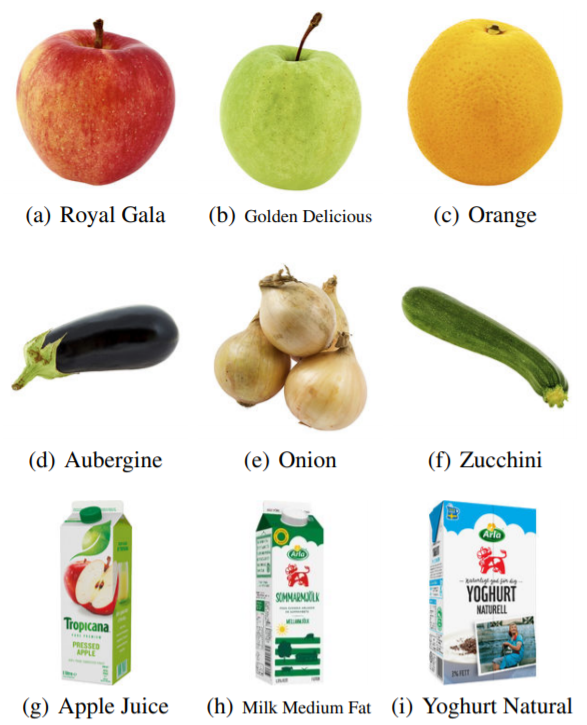
\includegraphics[scale=0.5]{PaperB/figures_and_tables/figure2.png}
    \caption{Examples of iconic images downloaded from a grocery shopping website, which corresponds to the target items in the images in Figure \ref{fig:dataset_figures}.}
    \label{fig:iconic_image_figures}
\end{figure}.
\end{comment}



For an image classification model to be capable of recognizing grocery items in the setting of grocery shopping, we need image data from grocery store environments. 
In our previous work~\citeB{B:klasson2019hierarchical}, we addressed this by collecting a novel dataset containing natural images of various raw grocery items and refrigerated products, where all images have been taken with a smartphone camera inside grocery stores to simulate a realistic shopping scenario.
In addition to the natural images, we also looked upon alternative types of grocery item data that could facilitate the classification task.
Grocery store chains commonly maintain websites where they store information about the grocery items they sell and are currently available in the store for online grocery shopping. 
For every item, there is usually an iconic image of the item with white background, a text description about the item, and also information about nutrition values, origin country, etc.
We downloaded such information from an online grocery shopping website to complement the natural images in the dataset.

To utilize the available information from the dataset for grocery item classification, we use a multi-view generative model Variational Canonical Correlation Analysis (VCCA)~\citeB{B:wang2016deep} that learns a shared representation of the natural images and the downloaded information. A view can be defined as any signal or data measured by some appropriate sensor and combining information from multiple views has previously been shown to be helpful for various image classification tasks~\citeB{B:donahue2015long-term, B:frome2013DeVISE, B:karpathy2015deep, B:kulkarni2013babytalk, B:lu2018neural, B:lu2016hierarchical, B:parikh2011relative, B:srivastava2014multimodal}. However, naively adding more additional information may not lead to improved results and even harm the performance of the model~\citeB{B:guler2014whats,B:ngiam2011multimodal}. We, therefore, perform an ablation study over the available views in the dataset with VCCA to gain insights into how each view can affect the classification performance. Moreover, VCCA allows separating the latent space into shared and private components, where the private latent spaces should hold information about a single view. This might prove useful for reducing view-specific noise in the shared latent space, which can ease the learning process of the representations we want to use for classification. We investigate the effects each view has on the learned representations of VCCA by measuring classification performances as well as visualizing the latent space for the different model settings. The contributions of this paper are the following:

\begin{itemize}
    \item We present a novel dataset with natural images of grocery items as well as iconic images and text descriptions for every item class (see subsection The Grocery Store Dataset in Results)~\citeB{B:klasson2019hierarchical}.
    %\ref{sec:grocery_store_dataset})~\citeB{klasson2019hierarchical}.
    The natural images are taken in grocery stores in different lighting conditions and backgrounds that can be challenging settings for a computer vision-based assistive device. The additional iconic images and text descriptions make the dataset suitable for multi-view learning by combining the natural images with the extra information to obtain better classification performance.  
    
    \item We investigate how to use information from different views for the task of grocery item classification with the deep generative model VCCA (see subsection Methods in Experimental Procedures).
    %\ref{sec:methods}).
    This model combines information from multiple views into a low-dimensional latent representation that can be used for classification. We also select a variant of VCCA denoted VCCA-private that separates shared and private information about each view through factorization of the latent representation (see subsection Extracting Private Information of Views with VCCA-private in Experimental Procedures). 
    %\ref{sec:extracting_private_information}). 
    Furthermore, we use a standard multi-view autoencoder model called Split Autoencoder (SplitAE)~\citeB{B:ngiam2011multimodal, B:wang2015deep} for benchmarking against VCCA and VCCA-private on classification.
    
    \item We conduct experiments with SplitAE, VCCA, and VCCA-private on the task of grocery item classification with our dataset (Results).
    %Section \ref{sec:results}).
    We perform a thorough ablation study over all views in the dataset to demonstrate how each view contributes to enhancing the classification performance and conclude that utilizing the web-scraped views yields better classification results than only using the natural images (see subsection Classification Results in Results).
    % Section \ref{sec:classification_results}). 
    To gain further insights into the results, we visualize the learned latent representations of the VCCA models and discuss how the iconic images and textual descriptions impose different structures on the latent space that are beneficial for classification (see subsection Investigation of the Learned Representations in Results).
    %Section \ref{sec:investigation_of_the_learned_representations}). 
    
\end{itemize}
This work is an extended version of Klasson \etal~\citeB{B:klasson2019hierarchical}, where we first presented this dataset. In this paper, we have added a validation set of natural images from two stores that were not present in the training and test set splits from \citeB{B:klasson2019hierarchical} to avoid overfitting effects. We also demonstrate how the text descriptions can be utilized alone and along with the iconic images in a multi-view setting, while \citeB{B:klasson2019hierarchical} only experimented with the combination of natural and iconic images to build better representations of grocery items. Finally, we decode iconic images from unseen natural images as an alternative to evaluate the usefulness of the latent representations (see subsection Decoding Iconic Images from Unseen Natural Images in Results).
%(see Section \ref{sec:decoding_iconic_images}). 
As we only evaluated the decoded iconic images qualitatively in Klasson \etal~\citeB{B:klasson2019hierarchical}, we have extended the assessment by comparing the quality of the decoded images from different VCCA models with multiple image similarity metrics. 

%% RELATED WORK
Next, we discuss image datasets, food datasets, and multi-view models related to our work:

\paragraph{Image Datasets} Many image datasets used in computer vision have been collected by downloading images from the web \citeB{B:deng2009imagenet, B:everingham2010pascal, B:gebru2017finegrained, B:griffin2007caltech256, B:krishna2016visualgenome, B:Krizhevsky2009cifar100, B:Lin2014MicrosoftCoco, B:nilsback2008flowers, B:song2016deep, B:WahCUB_200_2011, B:xiao2010sundatabase, B:young2014flickr30k}. 
Some datasets~\citeB{B:deng2009imagenet, B:griffin2007caltech256, B:Krizhevsky2009cifar100, B:nilsback2008flowers, B:WahCUB_200_2011} use search words with the object category in isolation, which typically returns high-quality images where the searched object is large and centered. To collect images from more real-world scenarios, searching for combinations of object categories usually returns images of two searched categories but also numerous other categories~\citeB{B:Lin2014MicrosoftCoco, B:young2014flickr30k}. 
The simplest annotation of these images is to provide a class label for the present objects. Occasionally, the dataset can use a hierarchical labeling structure and provide a fine- and coarse-grained label to objects where it is applicable. 
The annotators can also be asked to increase the possible level of supervision for the objects by, for instance, providing bounding boxes, segmentation masks, keypoints, text captions that describe the scene, and reference images of the objects~\citeB{B:gebru2017finegrained, B:krishna2016visualgenome, B:Lin2014MicrosoftCoco, B:nilsback2008flowers, B:WahCUB_200_2011, B:young2014flickr30k}. Our dataset includes reference (iconic) images of the objects that were web-scraped from a grocery store website. We also downloaded text descriptions that describe general attributes of the grocery items, such as flavor and texture, rather than the whole visual scene. The grocery items have also been labeled hierarchically in a fine- and coarse-grained manner if there exist multiple variants of specific items. For example, fine-grained classes of apples such as \textit{Golden Delicious} or \textit{Royal Gala} belongs to the coarse-grained class \textit{apple}.

\paragraph{Food Datasets} 
Recognizing grocery items in their natural environments, such as grocery stores, shelves, and kitchens, have been addressed in plenty of previous works \citeB{B:geng2018fine, B:george2014recognizing, B:hsiao2010making, B:jund2016freiburg, B:klasson2019hierarchical, B:lai2011large, B:merler2007recognizing, B:singh2014bigbird, B:waltner2015mango, B:wei2019rpc, B:winlock2010toward, B:yu2018take}. The addressed tasks range from hierarchical classification, object detection, segmentation, and 3D model generation. Most of these works collect a dataset that resembles shopping or cooking scenarios, where the datasets vary in the degree of labeling, different camera views, and the data domain difference between the training and test set. 
The training sets in GroZi-120~\citeB{B:merler2007recognizing}, Grocery Products~\citeB{B:george2014recognizing}, and CAPG-GP~\citeB{B:geng2018fine} datasets were obtained by web-scraping product images of single instances on grocery web stores, while the test sets were collected in grocery stores where there can be single and multiple instances of the same item and other different items.
The RPC~\citeB{B:wei2019rpc} and TGFS~\citeB{B:yu2018take} datasets are used for object detection and classification of grocery products, where RPC is targeted for automatic checkout systems and TGFS is for the task of recognizing items purchased from self-service vending machines.
The BigBIRD~\citeB{B:singh2014bigbird} dataset and datasets from~\citeB{B:hsiao2010making, lai2011large} contain images of grocery items from multiple camera views, segmentation masks, and depth maps for 3D reconstruction of various items. 
The Freiburg Groceries~\citeB{B:jund2016freiburg} dataset contains images taken with smartphone cameras of items inside grocery stores, while its test set consists of smartphone photos in home environments with single or multiple instances from different kinds of items. The dataset presented in~\citeB{B:waltner2015mango} also contains images taken with smartphone cameras inside grocery stores to develop a mobile application for recognizing raw food items and provide details about the item, such as nutrition values and recommendations of similar items. Other works that collected datasets of raw food items, such as fruits and vegetables, focused on the standard image classification task~\citeB{B:muresan2017fruit, B:marko2013fids30} and on detecting fruits in orchards for robotic harvesting~\citeB{B:bargoti2017deepfruitdetection, B:sa2016deepfruits}. Our dataset -- the Grocery Store dataset -- shares many similarities with the mentioned works above, for instance, that all images of groceries are taken in their natural environment, the hierarchical labeling of the classes, and the iconic product images for each item in the dataset. Additionally, we have provided a text description for each item that was web-scraped along with the iconic image. As most grocery item datasets only include packaged products, we have also collected images of different fruit and vegetable classes along with packages in our dataset. 

Other examples of food datasets are those with images of food dishes, where \citeB{B:min2019survey} provides a summary of existing benchmark food datasets. The contents of these datasets range from images of food dishes~\citeB{B:bossard2014food101, B:kawano2014automatic, B:min2019ingredient, B:rich2016towards}, cooking videos~\citeB{B:damen2018scaling}, recipes~\citeB{B:marin2019learning, B:salvador2017learning, B:yagcioglu2018recipeqa}, and also restaurant-oriented information~\citeB{B:beijbom2015menu, B:xu2015geolocalized}. One major difference between recognizing groceries and food dishes is the appearance of the object categories in the images. For instance, a fruit or vegetable is usually intact and present in the image, while ingredients that are significant for recognizing a food dish may not be visible at all depending on the recipe. However, recognizing raw food items and dishes share similarities since they can appear with many different visual features in the images compared to packaged groceries, e.g., carton boxes, cans, and bottles, where the object classes have identical shape and texture. 
Another key difference is the natural environments and scenes where the images of grocery items and food dishes have been taken. Food dish images usually show the food on a plate placed on a table and, occasionally, with cutlery and a glass next to the plate. Images taken in grocery stores can cover many instances of the same item stacked close to each other in shelves, baskets, and refrigerators, while there can be multiple different kinds of items next to each other in a kitchen environment. 
To summarize, recognizing grocery items and food dishes are both challenging tasks because examples from the same category can look very different and also appear in various realistic settings in images.


\paragraph{Multi-View Learning Models} There exist lots of multi-view learning approaches for data fusion of multiple features~\citeB{B:baltruvsaitis2018multimodal, B:cremer2018importance, B:frome2013DeVISE, B:fu2016semi, B:karpathy2015deep, B:ngiam2011multimodal, B:pieropan2014audio,  B:salzmann2010factorized, B:shi2019variational, B:suzuki2016joint, B:tsai2018learning, B:vedantam2017generative, B:wang2016deep, B:wu2018multimodal, B:xian2018zero, B:xu2013survey, B:zhang2016inter, B:zhao2017multi}. A common approach is to obtain a shared latent space for all views with the assumption that each view has been generated from this shared space~\citeB{B:xu2013survey}. A popular example of this is approach is Canonical Correlation Analysis (CCA)~\citeB{B:hotelling1936relations}, which aims to project two sets of variables (views) into a lower-dimensional space so that the correlation between the projections is maximized. Similar methods propose maximizing other alignment objectives for embedding the views, such as ranking losses~\citeB{B:frome2013DeVISE, B:fu2016semi, B:karpathy2015deep, B:xian2018zero}. 
There exist nonlinear extensions of CCA, e.g., Kernel CCA~\citeB{B:akaho2006kernel} and Deep CCA~\citeB{B:andrew2013deep}, that optimize their nonlinear feature mappings based on the CCA objective. 
Deep Canonically Correlated Autoencoders (DCCAE)~\citeB{B:wang2015deep} is a Deep CCA model with an autoencoding part, which aims to maximize the canonical correlation between the extracted features as well as reconstructing the input data. 
Removing the CCA objective reduces DCCAE to a standard multi-view autoencoder, e.g., Bimodal Autoencoders and Split Autoencoders (SplitAEs)~\citeB{B:ngiam2011multimodal, B:wang2015deep}, that only aim to learn a representation that best reconstructs the input data. SplitAEs aim to reconstruct two views from a representation encoded from one of the views. This approach was empirically shown to work better than Bimodal Autoencoders in \citeB{B:ngiam2011multimodal} in situations where only a single view is present at both training and test time.

Variational CCA (VCCA)~\citeB{B:wang2016deep} can be seen as an extension of CCA to deep generative models, but can also be described as a probabilistic version of SplitAEs.
VCCA uses the amortized inference procedure from Variational Autoencoders (VAEs)~\citeB{B:kingma2013auto, B:zhang2018advances} to learn the shared latent space by maximizing a lower bound on the data log-likelihood of the views. Succeeding works have proposed new learning objectives and inference methods for enabling conditional generation of views, e.g., generating an image conditioned on some text and vice versa~\citeB{B:cremer2018importance, B:shi2019variational, B:suzuki2016joint, B:vedantam2017generative, B:wu2018multimodal}. These approaches rely on fusing the views into the shared latent space as the inference procedure, which often requires tailored training and testing paradigms when views are missing. However, adding information from multiple views may not lead to improved results and can even make the model perform worse on the targeted task~\citeB{B:guler2014whats, B:ngiam2011multimodal}. This is especially the case when views have noisy observations, which complicates learning a shared latent space that combines the commonalities between the views. To avoid disturbing the shared latent space with noise from single views, some works design models which extend the shared latent space with private latent spaces for each view that should contain the view-specific variations to make learning the shared variations easier~\citeB{B:hyvarinen2000independent, B:salzmann2010factorized, B:tsai2018learning, B:wang2016deep, B:zhang2016inter}. VCCA can be extended to extract shared and private information between different views through factorization of the latent space into shared and private parts. In this paper, we investigate if the classification performance of grocery items in natural images can be improved by extracting the view-specific variations in the additional views (iconic images and product descriptions) from the shared latent space with this variant of VCCA called VCCA-private. We will experiment with treating each data point as pairs of natural images and either iconic images or text descriptions as well as triplets of natural images, iconic images, and text descriptions.
A difference between how we apply VCCA to our dataset compared to the works above is that the iconic image and text description are the same for every natural image of a specific class.  



